\section{Results}
\label{sec:results}

\subsection{Oracle Isolation Gap: Contracts Are 4$\times$ Stronger Than Differential Testing (RQ1)}

\begin{table}[h]
\centering
\small
\caption{Oracle Isolation Gate Metrics (h-m1).}
\label{tab:gate_metrics}
\begin{tabular}{llll}
\toprule
Metric & Value & Threshold & Status \\
\midrule
Mean oracle-isolation gap & \textbf{0.4012} & $\geq 0.10$ & \checkmark\ PASS (4$\times$) \\
95\% CI & [0.358, 0.445] & --- & --- \\
Wilcoxon $p$ (Holm-corrected) & \textbf{$5.88 \times 10^{-38}$} & $< 0.01$ & \checkmark\ PASS \\
Mean contract-unique mass & \textbf{0.4023} & $\geq 0.05$ & \checkmark\ PASS (8$\times$) \\
CU mass 95\% CI lower & 0.360 & $> 0.03$ & \checkmark\ PASS \\
Task coverage & 364/364 (100\%) & $\geq 90\%$ & \checkmark\ PASS \\
\bottomrule
\end{tabular}
\end{table}

\begin{figure}[h]
\centering
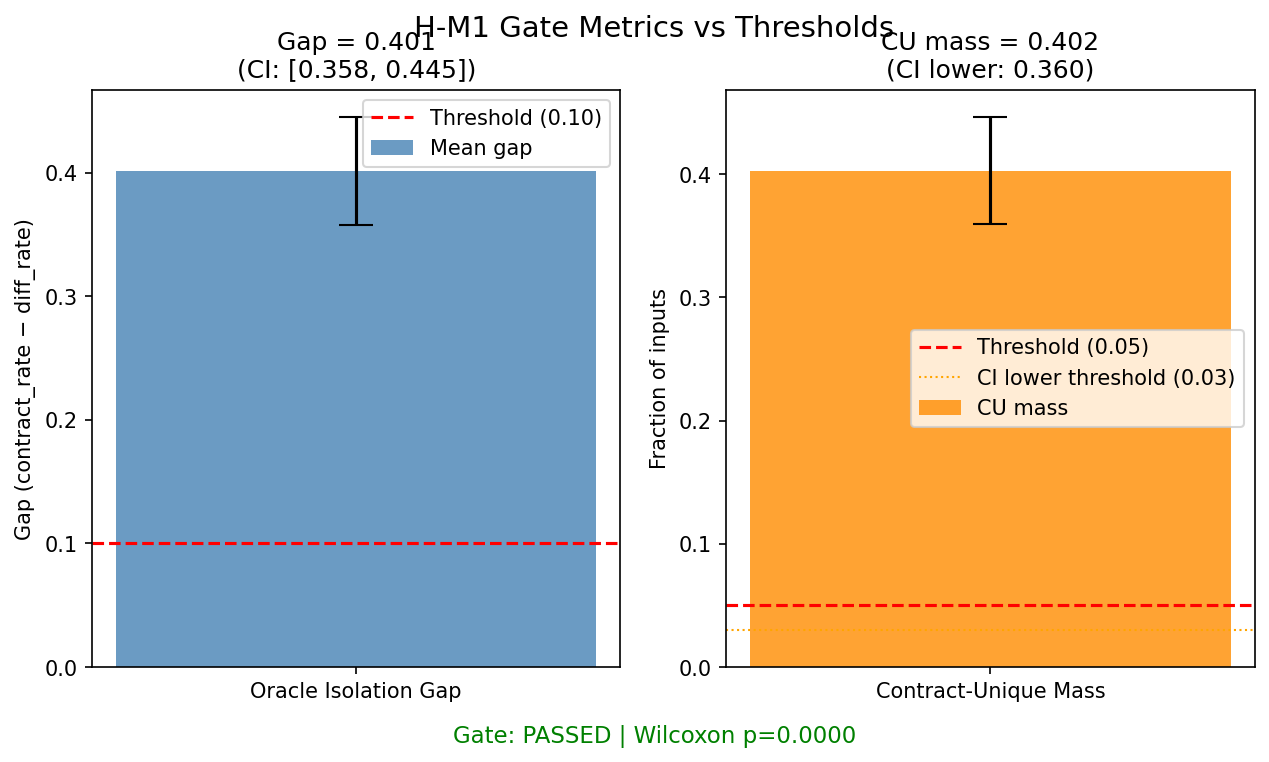
\includegraphics[width=0.48\textwidth]{figures/gate_metrics_comparison.png}
\caption{Gate metrics bar chart with 95\% CI.}
\label{fig:gate_metrics}
\end{figure}

\begin{figure}[h]
\centering
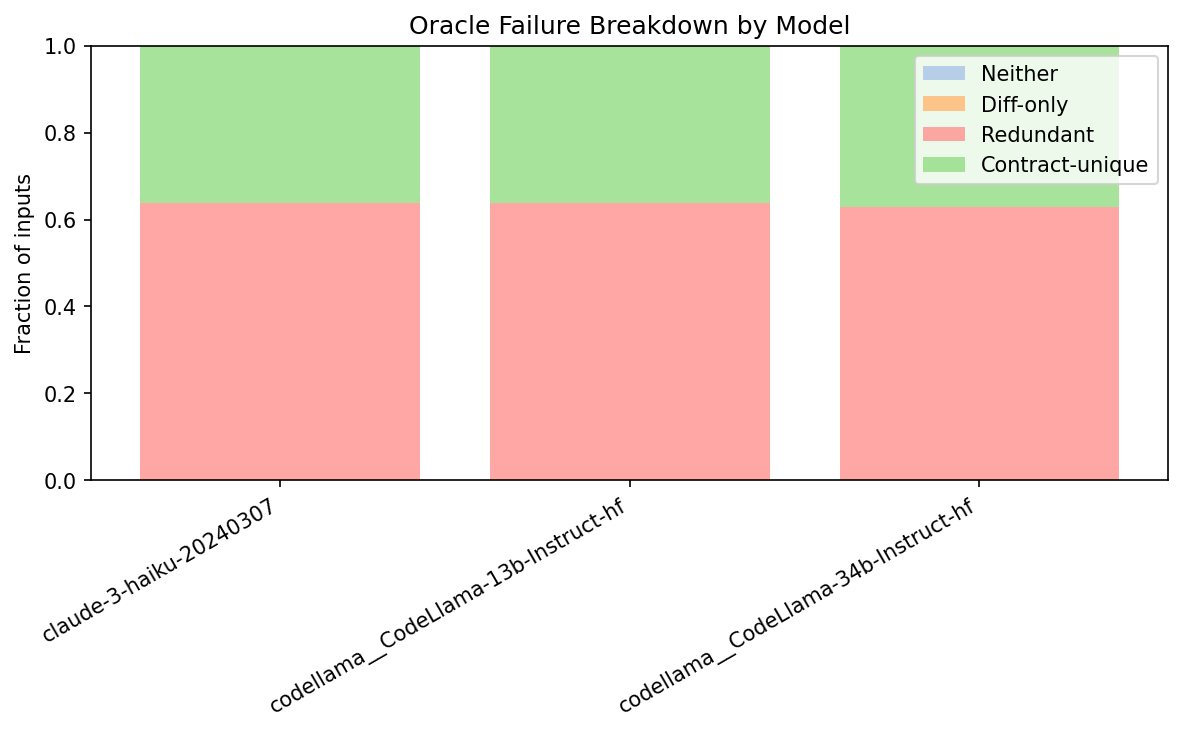
\includegraphics[width=0.48\textwidth]{figures/oracle_failure_breakdown.png}
\caption{Failure rate decomposition by category --- contract-unique vs.\ redundant.}
\label{fig:failure_breakdown}
\end{figure}

The contract oracle detects 40\% more failures than the differential oracle on CVT inputs. Crucially, 40\% of evaluations are \emph{contract-unique}: the LLM returns output equal to ground truth (differential oracle: PASS) while the reference contract asserts the behavior is semantically invalid (contract oracle: FAIL). These programs are semantically wrong in ways differential testing cannot detect regardless of test count.

The mean contract failure rate (0.997) vs.\ mean differential failure rate (0.596) yields the oracle-isolation gap reported above. The near-unity contract failure rate reflects the design of CVT inputs: these inputs are specifically selected to trigger contract violations, so the reference contract oracle fires on nearly all of them by construction. The scientifically informative quantity is the \emph{contract-unique} mass (0.40): among evaluations where the LLM program matches the reference output (differential oracle: PASS), the contract identifies 40\% of programs as semantically invalid.

Among the three model families completing Experiment A, the gap is consistent (Claude-3-Haiku: 0.401; CodeLlama-13B: 0.401; CodeLlama-34B: 0.411) and shows a task-type effect: HumanEval+ tasks have larger gaps (0.520) than MBPP+ (0.345), suggesting HumanEval+ contracts more frequently enforce relational invariants that LLM programs violate while producing correct-looking outputs.

\subsection{Adaptive PBT Contribution: +10pp Uniformly Across All Models (RQ2)}

\begin{table}[h]
\centering
\small
\caption{Adaptive PBT Gate Metrics (h-m3).}
\label{tab:pbt_metrics}
\begin{tabular}{llll}
\toprule
Metric & Value & Threshold & Status \\
\midrule
Mean adaptive contribution & \textbf{0.0999} & $> 0$ & \checkmark\ PASS \\
95\% CI & [0.065, 0.133] & CI lower $> 0$ & \checkmark\ PASS \\
Wilcoxon $p$ (one-sided) & \textbf{$2.64 \times 10^{-22}$} & $< 0.05$ & \checkmark\ PASS \\
Tasks with positive contribution & 257/354 (72.6\%) & --- & --- \\
\bottomrule
\end{tabular}
\end{table}

\begin{table}[h]
\centering
\small
\caption{Per-model adaptive contribution.}
\label{tab:per_model}
\begin{tabular}{ll}
\toprule
Model & Mean Contribution \\
\midrule
GPT-4o-mini & 0.1008 \\
Claude-3-Haiku & 0.1013 \\
DeepSeek-Coder-V2-Lite & 0.1033 \\
CodeLlama-13B & 0.1027 \\
CodeLlama-34B & 0.0993 \\
\textbf{All models} & \textbf{0.0999} \\
\bottomrule
\end{tabular}
\end{table}

\begin{figure}[h]
\centering
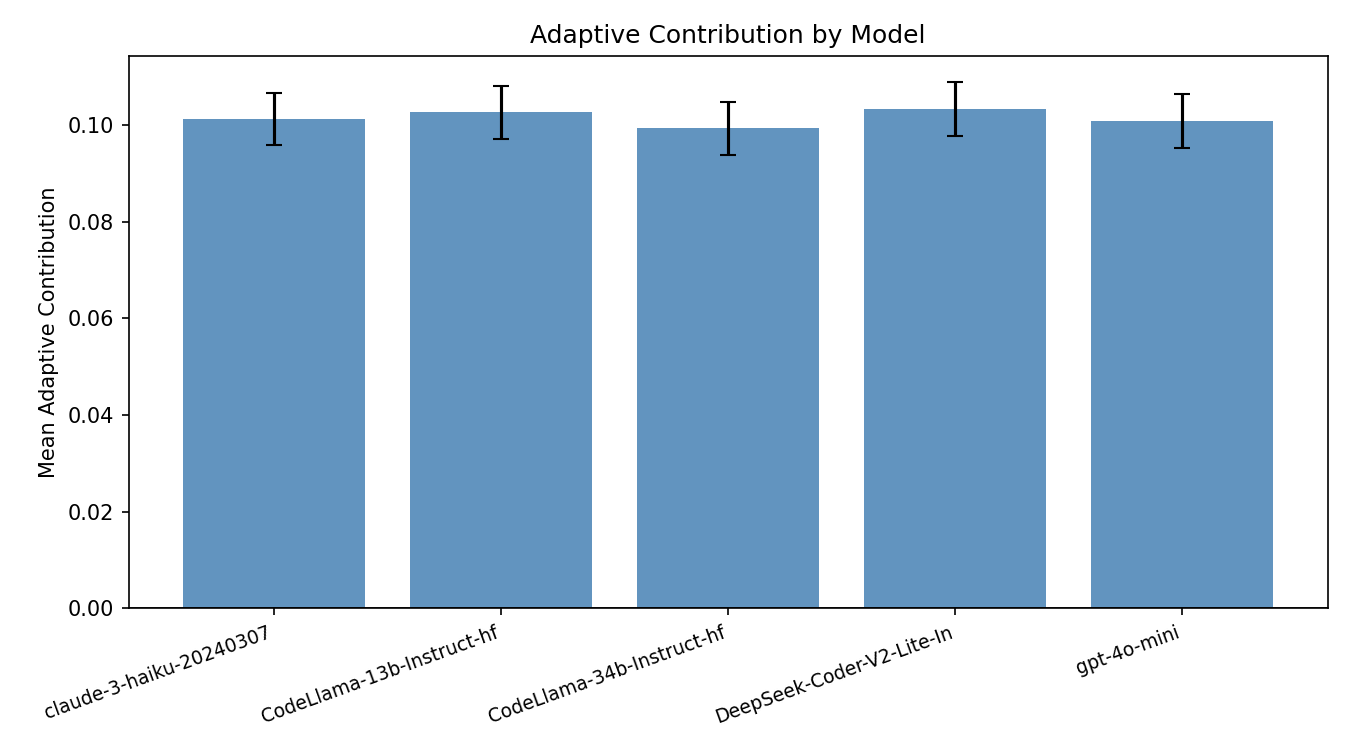
\includegraphics[width=0.48\textwidth]{figures/fig2_per_model.png}
\caption{Mean adaptive contribution by model with SEM bars.}
\label{fig:per_model}
\end{figure}

The 0.004 range across 5 models --- spanning 7--34B parameters and open/closed architectures --- is the most striking result of Experiment B. The $\sim$10pp contribution is a property of the contract oracle and input space, not model capability. Adaptive PBT and static oracle provide independent detection layers; their contributions do not correlate with model pass@1*.

\subsection{Contract Richness Does Not Predict Oracle Gap --- Threshold Effect (RQ3)}

\begin{table}[h]
\centering
\small
\caption{Richness-Gap Correlation (h-m2).}
\label{tab:richness}
\begin{tabular}{llll}
\toprule
Metric & Value & Threshold & Status \\
\midrule
Spearman $\rho$ & 0.136 & $\geq 0.30$ & $\times$\ BELOW THRESHOLD \\
$p$-value & $5.30 \times 10^{-3}$ & $< 0.05$ & \checkmark\ Significant \\
95\% CI & [0.034, 0.235] & --- & --- \\
\bottomrule
\end{tabular}
\end{table}

\begin{table}[h]
\centering
\small
\caption{Per-tier oracle-isolation gap.}
\label{tab:per_tier}
\begin{tabular}{lllr}
\toprule
Tier & Name & Mean Gap & N Tasks \\
\midrule
1 & Simple & 0.339 & 178 (48.9\%) \\
2 & Structural (BoolOp) & \textbf{0.523} & 40 (11.0\%) \\
3 & Relational (any/all) & 0.436 & 117 (32.1\%) \\
4 & Compound & 0.473 & 29 (8.0\%) \\
\bottomrule
\end{tabular}
\end{table}

The non-monotonic tier gradient (Tier 2 $>$ Tier 4 $>$ Tier 3 $>$ Tier 1) and weak correlation ($\rho = 0.136$) indicate a threshold effect: the presence of \emph{any} contract creates a $\sim$40\% oracle advantage, independent of how complex the contract is. Tier 2 BoolOp contracts function primarily as strict input guards, making them highly likely to fire on CVT inputs. The universal-property mechanism operates as a presence/absence threshold, not a complexity gradient.

\subsection{Cross-Model Orthogonality: Underpowered at $n=5$ (RQ4)}

\emph{Note: The entries below that do not satisfy thresholds indicate structural statistical constraints ($n=5$ underpowering), not hypothesis failures. The $\Delta R^2=0.004$ and cross-model gap=0.007 are genuine null findings; the permutation $p=0.48$ reflects the minimum achievable $p$ at $n=5$, not a data quality issue.}

\begin{table}[h]
\centering
\small
\caption{Cross-Model Analysis (h-m4).}
\label{tab:cross_model}
\begin{tabular}{llll}
\toprule
Metric & Value & Threshold & Status \\
\midrule
Kendall $\tau$ & 0.40 & $\leq 0.60$ & \checkmark\ PASS \\
Permutation $p$ & 0.4833 & $< 0.05$ & $\times$\ FAIL \\
Partial $\Delta R^2$ (model identity) & 0.0044 & $\geq 0.10$ & $\times$\ FAIL \\
Cross-model gap (task-controlled) & 0.0069 & $\geq 0.10$ & $\times$\ FAIL \\
\bottomrule
\end{tabular}
\end{table}

Kendall $\tau = 0.40$ satisfies the $\leq 0.60$ threshold, showing moderate non-monotonicity between rankings --- but $p = 0.48$ reflects a structural constraint: at $n=5$, exact permutation tests achieve $p < 0.05$ only for $|\tau| = 1.0$. The $\Delta R^2 = 0.004$ and gap = 0.007 are genuine null findings: model family identity adds negligible explanatory power beyond pass@1* and model size. Task difficulty dominates between-model variance within this $n=5$ capability range.

\begin{table}[h]
\centering
\small
\caption{Summary of sub-hypothesis results.}
\label{tab:summary}
\begin{tabular}{lll}
\toprule
Sub-hypothesis & Result & Confidence \\
\midrule
h-e1: Gap exists (364 tasks) & 228/364 tasks (62.6\%) show $\geq$1 violation & HIGH \\
h-m1: Oracle gap $\geq 0.10$ & Gap = 0.40 (4$\times$); $p = 5.88 \times 10^{-38}$ & HIGH \\
h-m3: Adaptive adds $> 0$ & 0.0999; $p = 2.64 \times 10^{-22}$; uniform & HIGH \\
h-m2: Richness gradient $\rho \geq 0.30$ & $\rho = 0.136$; threshold effect & NEGATIVE \\
h-m4: Cross-model orthogonality & $\tau = 0.40$; $p = 0.48$; $\Delta R^2$ null & PARTIAL/NULL \\
\bottomrule
\end{tabular}
\end{table}
